\documentclass[a4paper, 12pt]{article}
\usepackage[T2A]{fontenc}
\usepackage[utf8]{inputenc}
\usepackage[english,russian]{babel}
\usepackage{amsmath, amsfonts, amssymb, amsthm, mathtools, misccorr, indentfirst, multirow}
\usepackage{wrapfig}
\usepackage{graphicx}
\usepackage{subfig}
\usepackage{adjustbox}
\usepackage{pgfplots}
\usepackage{wasysym}

\usepackage{geometry}
\geometry{top=20mm}
\geometry{bottom=20mm}
\geometry{left=20mm}
\geometry{right=20mm}
\newcommand{\angstrom}{\textup{\AA}}

\begin{document}
	\title{Изучение особенностей возбуждения и распространения акустических волн СВЧ в твердых телах}
	\author{Нехаев Александр 654 гр.}
	\date{\today}
	\maketitle
	\paragraph{Цель работы:}
	Снять частоту, зависимость коэффициента затухания амплитуды. Определить константы упругости 2 - го порядка.
	\section{Теоретическое введение}
	Под затуханием ультразвуковых волн (УЗВ) обычно понимают уменьшение интенсивности вдоль пути ее распространения. Это связано со следующими процессами: поглощением энергии УЗВ и переходом ее в тепло, с рассеянием на неоднородностях и причинами, сиоздающими кажущееся поглощение, связанное с методикой измерений, к примеру, разориентации образца относительно основных кристаллографических осей, дифракционные потери, потери из-за непараллельности торцевых граней образца и другие.

Первые две причины создают уменьшение интенсивности, пропорциональные самой интенсивности, то есть $-dI(x)=\gamma I(x)dx$ или $I(x)=I_{0}e^{-\gamma x}$. Для амплитуд выражение имеет вид $U(x)=U_{0}e^{-\alpha x}$. $U_{0}, I_{0}$ – интенсивность и амплитуда УЗВ во вхрдном сечении кристалла. $\alpha$ – коэффициент затухания амплитуды, а $\gamma=2\alpha$ – коэффициент затухания интенсивности. Если при измерении затухания амплитудные характеристики линейны, то для определения $\alpha$ можно использовать следующее выражение:
\begin{equation*}
\alpha=-\frac{1}{x_{1}-x_{2}}ln\frac{U(x_{1})}{U(x_{2})}
\end{equation*}
Если регистрация амплитуды УЗВ происходит в одном и том же сечении образца, то $x_{2}-x_{1}=2L$, где $L$ – длина образца, а величину можно найти, измеряя отношение амплитуд соответствующих импульсов на экране осциллографа. На этом и основа реализуемый в работе метод.

В работе на одном из двух торцов образца мы возбуждаем УЗВ, распространяющиеся вглубь образца. Переменное электрическое поле прикладывается к преобразователю на очень короткое время (порядка нескольких микросекунд). В результате по кристаллу распространяется короткий цуг УЗВ длиной $V_{s}\tau_{\text{имп}}$, где $V_{s}$ – скорость УЗВ. Испытав отражение от параллетьной грани и придя обратно, цуг вызывает но обкладках преобразователя переменное напряжение с частотой УЗВ. На выходе мы наблюдаем импульс длиной $\tau_{\text{имп}}$. Скорость УЗВ мы находим временную задержку n-го импульса относительно m-го. Эта задержка соответствует целому числу двойных пробегов цуга УЗВ вдоль образца, поэтому $V_{s}=\frac{2L(m-n)}{T_{3}}$.
	\section{Экспериментальная установка}
	\begin{figure}[!htb]
		\centering
		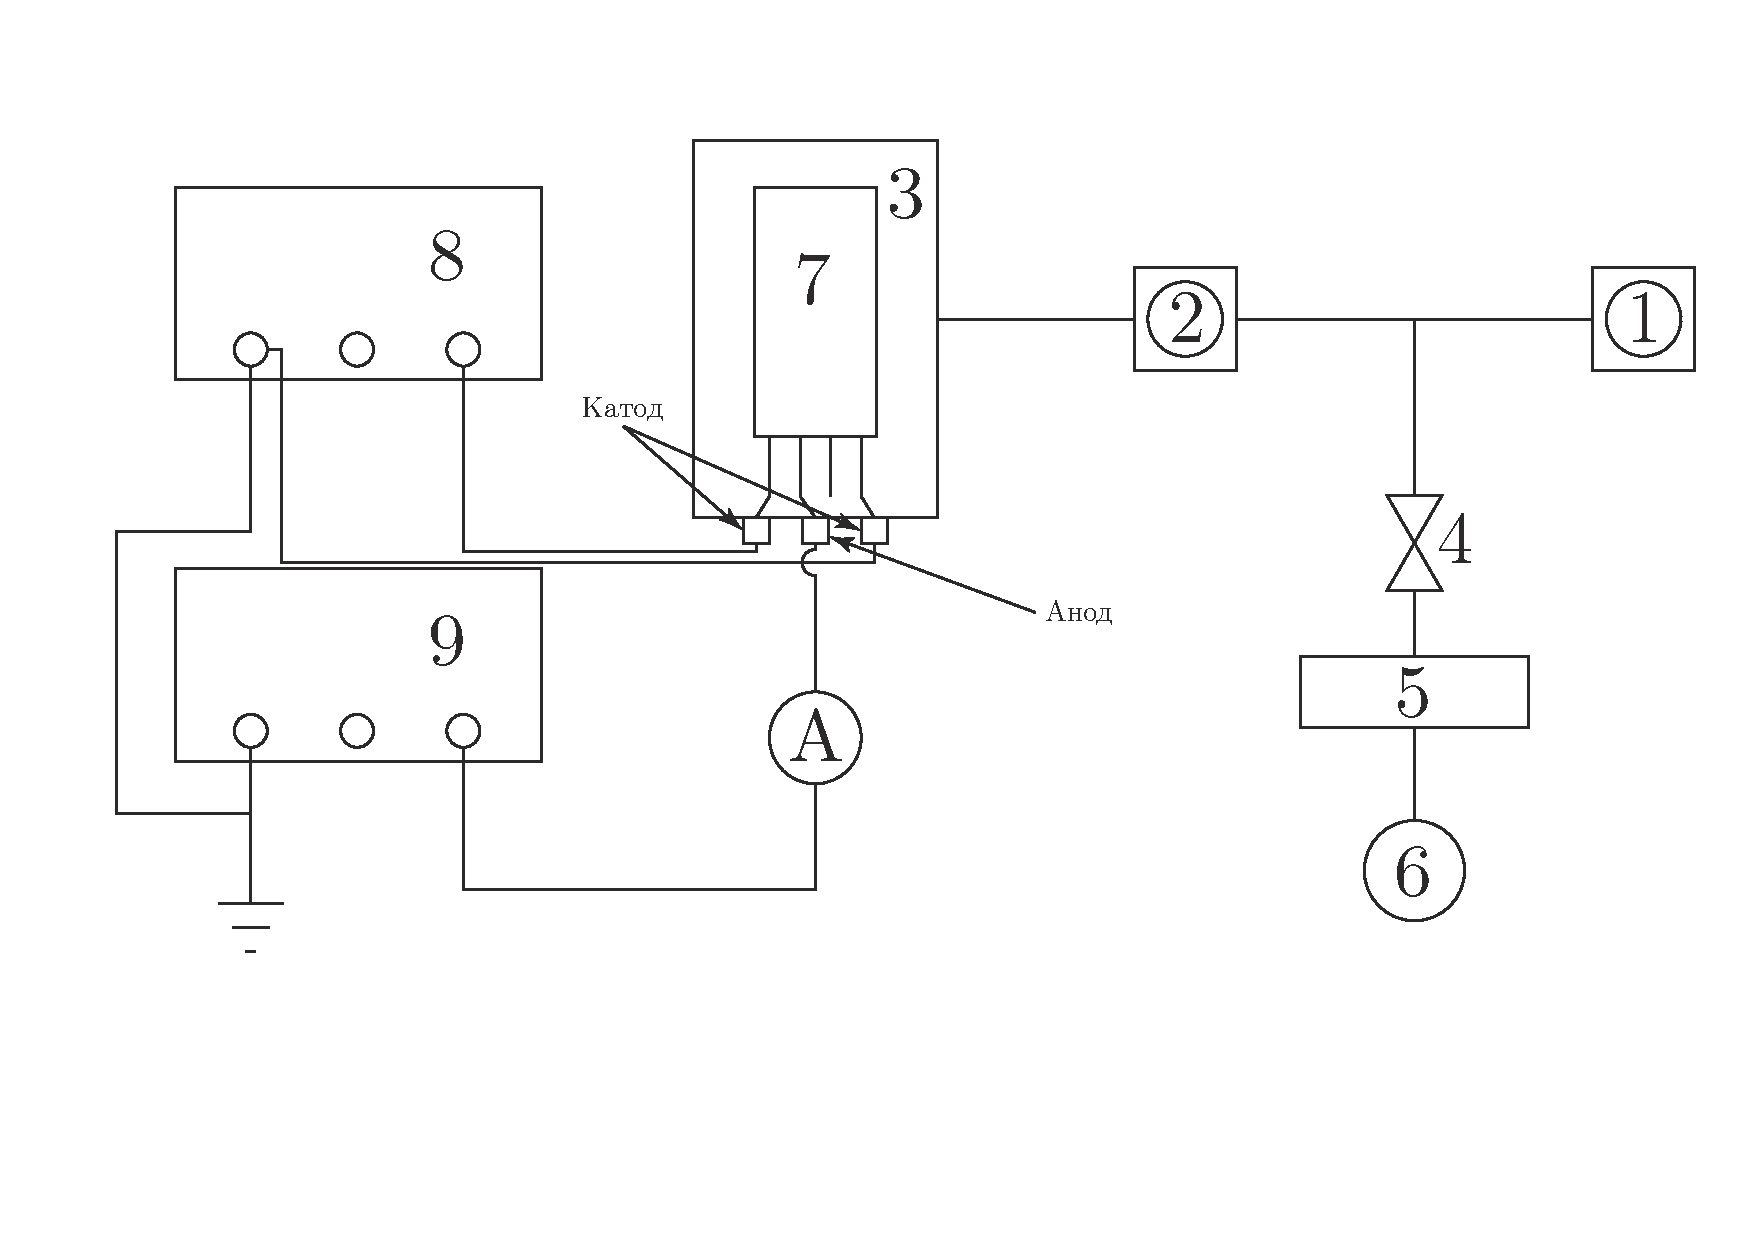
\includegraphics[scale=0.7]{PDF/scheme.pdf}
		\caption{Схема установки}
	\end{figure}
	\section{Ход работы}
	\begin{enumerate}
		\item Сняли частотную зависимость $\alpha(v)$ в кристалле SiO$_2$.
		\begin{table}[!htb]
			\centering
			\begin{tabular}{|c|c|c|c|}
				\hline
				$V$, МГц & $U_1$, В & $U_2$, В & $\alpha$, см$^{-1}$\\
				\hline
				430 & 1 & 2.1 & 0.555174\\
				500 & 3.4 & 5 & 0.288582\\
				600 & 3 & 5.8 & 0.493298\\
				700 & 2 & 4.2 & 0.555174\\
				800 & 1.6 & 4 & 0.685638\\
				980 & 0.8 & 3.7 & 1.14597\\
				\hline
			\end{tabular}
		\end{table}
		\item Полученная зависимость показана на графике.
		\begin{figure}[!htb]
			\centering
			\includegraphics[width=\textwidth]{graph.pdf}
			\caption{Зависимость $\alpha(v)$}
		\end{figure}
		Параметры образца:
		$L=2.9$ см, $t=54/7$ с.
		\item Проведем расчет $\Delta_{\text{диф}}$ на $v=400$ МГц по формуле:
		\begin{equation}
			\Delta_{\text{диф}}=20 \log(\frac{\lambda l}{\pi a^2})\cdot\frac{\sin(\frac{\lambda l}{\pi a^2}\cdot\frac{\pi}{3.83})^4}{(\frac{\lambda l}{\pi a^2}\cdot\frac{\pi}{3.83})^4}
		\end{equation}
		Радиус преобразователя приближенно равен:
		$a=0.05$ см, $l=2 L$, $\lambda_{\text{з}}=\frac{l/t}{400\text{МГц}}=-269.752$
		\item Определим скорость УЗВ в кристалле
		$v=\frac{2L}{t}=0.75$ см/с.
		Считая, что мы измерили скорость продольной волны, вычислили один из коэффициентов тензора модулей упругости:
		Значение плотности $\rho=2196$ кг/м$^3$ для SiO$_2$.
		$C_{11}=\rho*v^2=0.124136$ кг/(м*с$^2$).
	\end{enumerate}
	\section{Вывод}
	Сняли частотную характеристику коэффициента затухания амплитуды УЗВ в кристалле SiO$_2$. Определили скорость распространения УЗВ в кристалле SiO$_2$. Определили константу упругости 2-го порядка, оценили дифракционные потери в кристалле SiO$_2$.
\end{document}